\documentclass[UTF8,AutoFakeBold]{article}%支持粗体
\usepackage{ctex}
\usepackage{soul}
\usepackage{color}
\usepackage{geometry}   % 页边距调整
\usepackage{setspace}   % 行距调整
\usepackage{graphicx}   % 图片支持
\usepackage{float}      % 图片强制放置
\usepackage{xcolor}     % 代码着色
\usepackage{listings}   % 代码支持
\usepackage{indentfirst}% 首行缩进
\usepackage{titlesec}   % 设置标题
\usepackage{zhnumber}   % 设置中文section序号
\usepackage{amsmath,amssymb}    % 数学公式
\usepackage{enumerate, enumitem}
\usepackage{romannum}
\usepackage{multirow}
\usepackage{caption}
\captionsetup[figure]{labelsep=space} % 图编号与标题之间用空格
\usepackage{booktabs}   % 三线表
\usepackage{tabularx}   % 自动列宽表格
\usepackage{appendix}
\usepackage[super,square,sort&compress]{natbib}  % 文献管理宏包
\usepackage[colorlinks=true,
            linkcolor=black,
            citecolor=black,
            urlcolor=black]{hyperref}
\usepackage{subcaption}
\usepackage{textcomp}

% 页边距调整
\geometry{
	a4paper,
	left=2.54cm,
	right=1.5cm,
	top=2.0cm,
	bottom=2.54cm
}

% 定义简易代码框风格
\lstdefinestyle{simplebox}{
    backgroundcolor=\color{gray!10}, % 浅灰背景
    frame=single,                    % 单线边框
    rulecolor=\color{black},         % 边框颜色
    basicstyle=\ttfamily\small,      % 等宽字体
    keywordstyle=\color{blue},       % 关键字高亮
    commentstyle=\color{green!50!black}, % 注释样式
    stringstyle=\color{red!60!black},    % 字符串样式
    breaklines=true,                 % 自动换行
    numbers=left,                    % 行号在左侧
    numberstyle=\tiny\color{gray},   % 行号样式
    xleftmargin=2em,                 % 左边距
    framexleftmargin=2em,            % 行号与代码间隔
}

% 一级标题：一、
\renewcommand{\thesection}{\zhnum{section}、}
\titleformat{\section}{\Large\bfseries\songti}{\thesection}{0em}{}

% 二级标题：（一）
\renewcommand{\thesubsection}{（\chinese{subsection}）}
\titleformat{\subsection}{\large\bfseries\songti}{\thesubsection}{0.5em}{}

% 三级标题：1.
\renewcommand{\thesubsubsection}{\arabic{subsubsection}.}
\titleformat{\subsubsection}{\normalsize\bfseries\songti}{\thesubsubsection}{0.5em}{}

% 行距调整
\linespread{1}
% 首行缩进
\setlength{\parindent}{2em}
% 代码块命令
\setmonofont{Consolas}
\definecolor{codeBgColor}{RGB}{249, 242, 244}
\definecolor{codeTextColor}{RGB}{202, 37, 78}
\newcommand{\linecode}[1]{
    \begingroup
    \sethlcolor{codeBgColor}
    \fontsize{9pt}{\baselineskip}\ttfamily\textcolor{codeTextColor}{\hl{\,#1\,}}
    \endgroup
}
\newcommand{\boldit}[1]{\textbf{\textit{#1}}}

\begin{document}
\pagenumbering{arabic}%设置页码

% ====================== 报告抬头 ======================
\begin{figure}[t]
    \centering
    
\includegraphics[width=9.3cm]{resource/head.jpg}
    \qquad\qquad
    \parbox[b]{4.5cm}{
        专业：\underline{\hbox to 0.75\linewidth{\hfill 生物医学工程\hfill}}\\

        \vspace{-1.5ex}
        姓名：\underline{\hbox to 0.75\linewidth{\hfill 刘博涵\hfill}}\\

        \vspace{-1.5ex}
        学号：\underline{\hbox to 0.75\linewidth{\hfill 3250105988\hfill}}\\

        \vspace{-1.5ex}
        日期：\underline{\hbox to 0.75\linewidth{\hfill 2026.xx.xx \hfill}}\\

        \vspace{-1.5ex}
        地点：\underline{\hbox to 0.75\linewidth{\hfill 东三-211 \hfill}}\\
    }
\end{figure}
\vspace{6ex}
\parbox{1\linewidth}{
    \renewcommand{\baselinestretch}{1.2}\selectfont % 设置行距 1.2 倍
    课程名称：\underline{\hbox to 0.30\linewidth{\hfill 电路与模拟电子技术实验\hfill}}
    指导老师：\underline{\hbox to 0.17\linewidth{\hfill 周晶\hfill}}
    成绩：\underline{\hbox to 0.15\linewidth{\hfill \hfill}}\\
    实验名称：\underline{\hbox to 0.35\linewidth{\hfill xxx \hfill}}
    实验类型：\underline{\hbox to 0.34\linewidth{\hfill 模拟电子技术实验\hfill}}
}
\vspace*{6ex}

% =====================================================
% 模板说明（正式提交前请删除本说明框）：
% 1. 本模板共七个章节，其中标注“必填”的章节不可缺少，
%    其余章节如无内容可写“无”，但不建议删除标题。
% 2. 括号内的灰色指导文字仅起提示作用，正式报告中请替换
%    为自己的内容，切勿原样保留。
% 3. 数据记录、处理与不确定度评定须严格遵照
%    data/数据处理准则.md（与大学物理实验准则有差异）。
% 4. 编译方式：XeLaTeX，含参考文献时按
%    XeLaTeX → BibTeX → XeLaTeX → XeLaTeX 顺序编译。
% =====================================================

% ====================== 一、实验目的和要求 ======================
\section{实验目的和要求（必填）}
（写明本次实验要达到的目的，以及实验的具体要求；分条列出）

\begin{itemize}
  \item 
  \item 
  \item 
\end{itemize}

% ====================== 二、实验内容和原理 ======================
\section{实验内容和原理（必填）}
（简述本次实验所做的内容；完整叙述实验原理，包括必要的电路图、原理图、波形图、公式及必要推导。
多个实验项目可分别用 \verb|\subsection| 列出。）

\subsection{实验项目一：\textit{（填写项目名称）}}

\subsubsection{实验原理}
（在此阐述工作原理，给出公式及推导。行内公式示例：$I = U/R$；
带编号的行间公式示例如下。）

\begin{equation}
    y = f(x_1,x_2,\dots,x_m)
    \label{eq:example}
\end{equation}

\subsubsection{实验电路}
（在此插入电路图或原理图，图片放在 resource/ 目录，单图/双图写法见文末“插图模板”。）

% \begin{figure}[H]
%   \centering
%   \includegraphics[width=0.6\textwidth]{resource/xxx.png}
%   \caption{电路图（写明图名）}
%   \label{fig:circuit}
% \end{figure}

% ====================== 三、主要仪器设备 ======================
\section{主要仪器设备（必填）}
（列出实验所用仪器仪表及元器件的名称、型号、规格参数与数量，如下表；内容较少时也可分条列出。）

\begin{table}[H]
  \centering
  \caption{主要仪器设备一览表}
  \label{tab:instruments}
  \renewcommand{\arraystretch}{1.25}
  \begin{tabular}{c l l c}
    \toprule
    序号 & 仪器名称及型号 & 规格参数 & 数量 \\
    \midrule
    1 & （如：数字万用表 UT890D+） & （如：直流电压档 $\dots$） & 1 \\
    2 &  &  &  \\
    3 &  &  &  \\
    \bottomrule
  \end{tabular}
\end{table}

% ====================== 四、操作方法和实验步骤 ======================
\section{操作方法和实验步骤}
（按操作先后顺序写明：实验电路的连接与检查、仪器仪表的设置与调试、测量操作过程；
可配接线图或实验过程照片。步骤须具体、可复现。）

\begin{enumerate}[label=（\arabic*）]
  \item 
  \item 
  \item 
\end{enumerate}

% ====================== 五、实验数据记录和处理 ======================
\section{实验数据记录和处理}
（1. 完整记录原始数据；
2. 用表格整理数据，注明电路变量名称与单位，数值按有效数字规范书写；
3. 写明数据处理方法、计算公式与完整计算过程；
4. 插入处理后得到的曲线、拟合图。数据处理须遵照《数据处理准则》。）

\subsection{原始数据记录}
% （方式一：粘贴原始记录纸照片）
% \begin{figure}[H]
%   \centering
%   \includegraphics[width=0.7\textwidth]{resource/原始记录.jpg}
%   \caption{原始数据记录（教师签字）}
% \end{figure}

（方式二：用三线表记录，示例如下。）

\begin{table}[H]
  \centering
  \caption{\textit{（填写数据表名称，如：二极管正向伏安特性测量数据）}}
  \label{tab:rawdata}
  \renewcommand{\arraystretch}{1.25}
  \begin{tabular}{c c c c c}
    \toprule
    序号 & 测量量 1\ /\ 单位 & 测量量 2\ /\ 单位 & 计算量\ /\ 单位 & 备注 \\
    \midrule
    1 &  &  &  &  \\
    2 &  &  &  &  \\
    3 &  &  &  &  \\
    \bottomrule
  \end{tabular}
\end{table}

\subsection{数据处理过程}
（写明所用处理方法——列表法、作图法或最小二乘拟合（本课程一般不用逐差法）；
列出计算公式、代入数据与计算结果；不确定度评定写出 A 类、B 类分量及合成过程。）

% 处理得到的曲线图可插入此处：
% \begin{figure}[H]
%   \centering
%   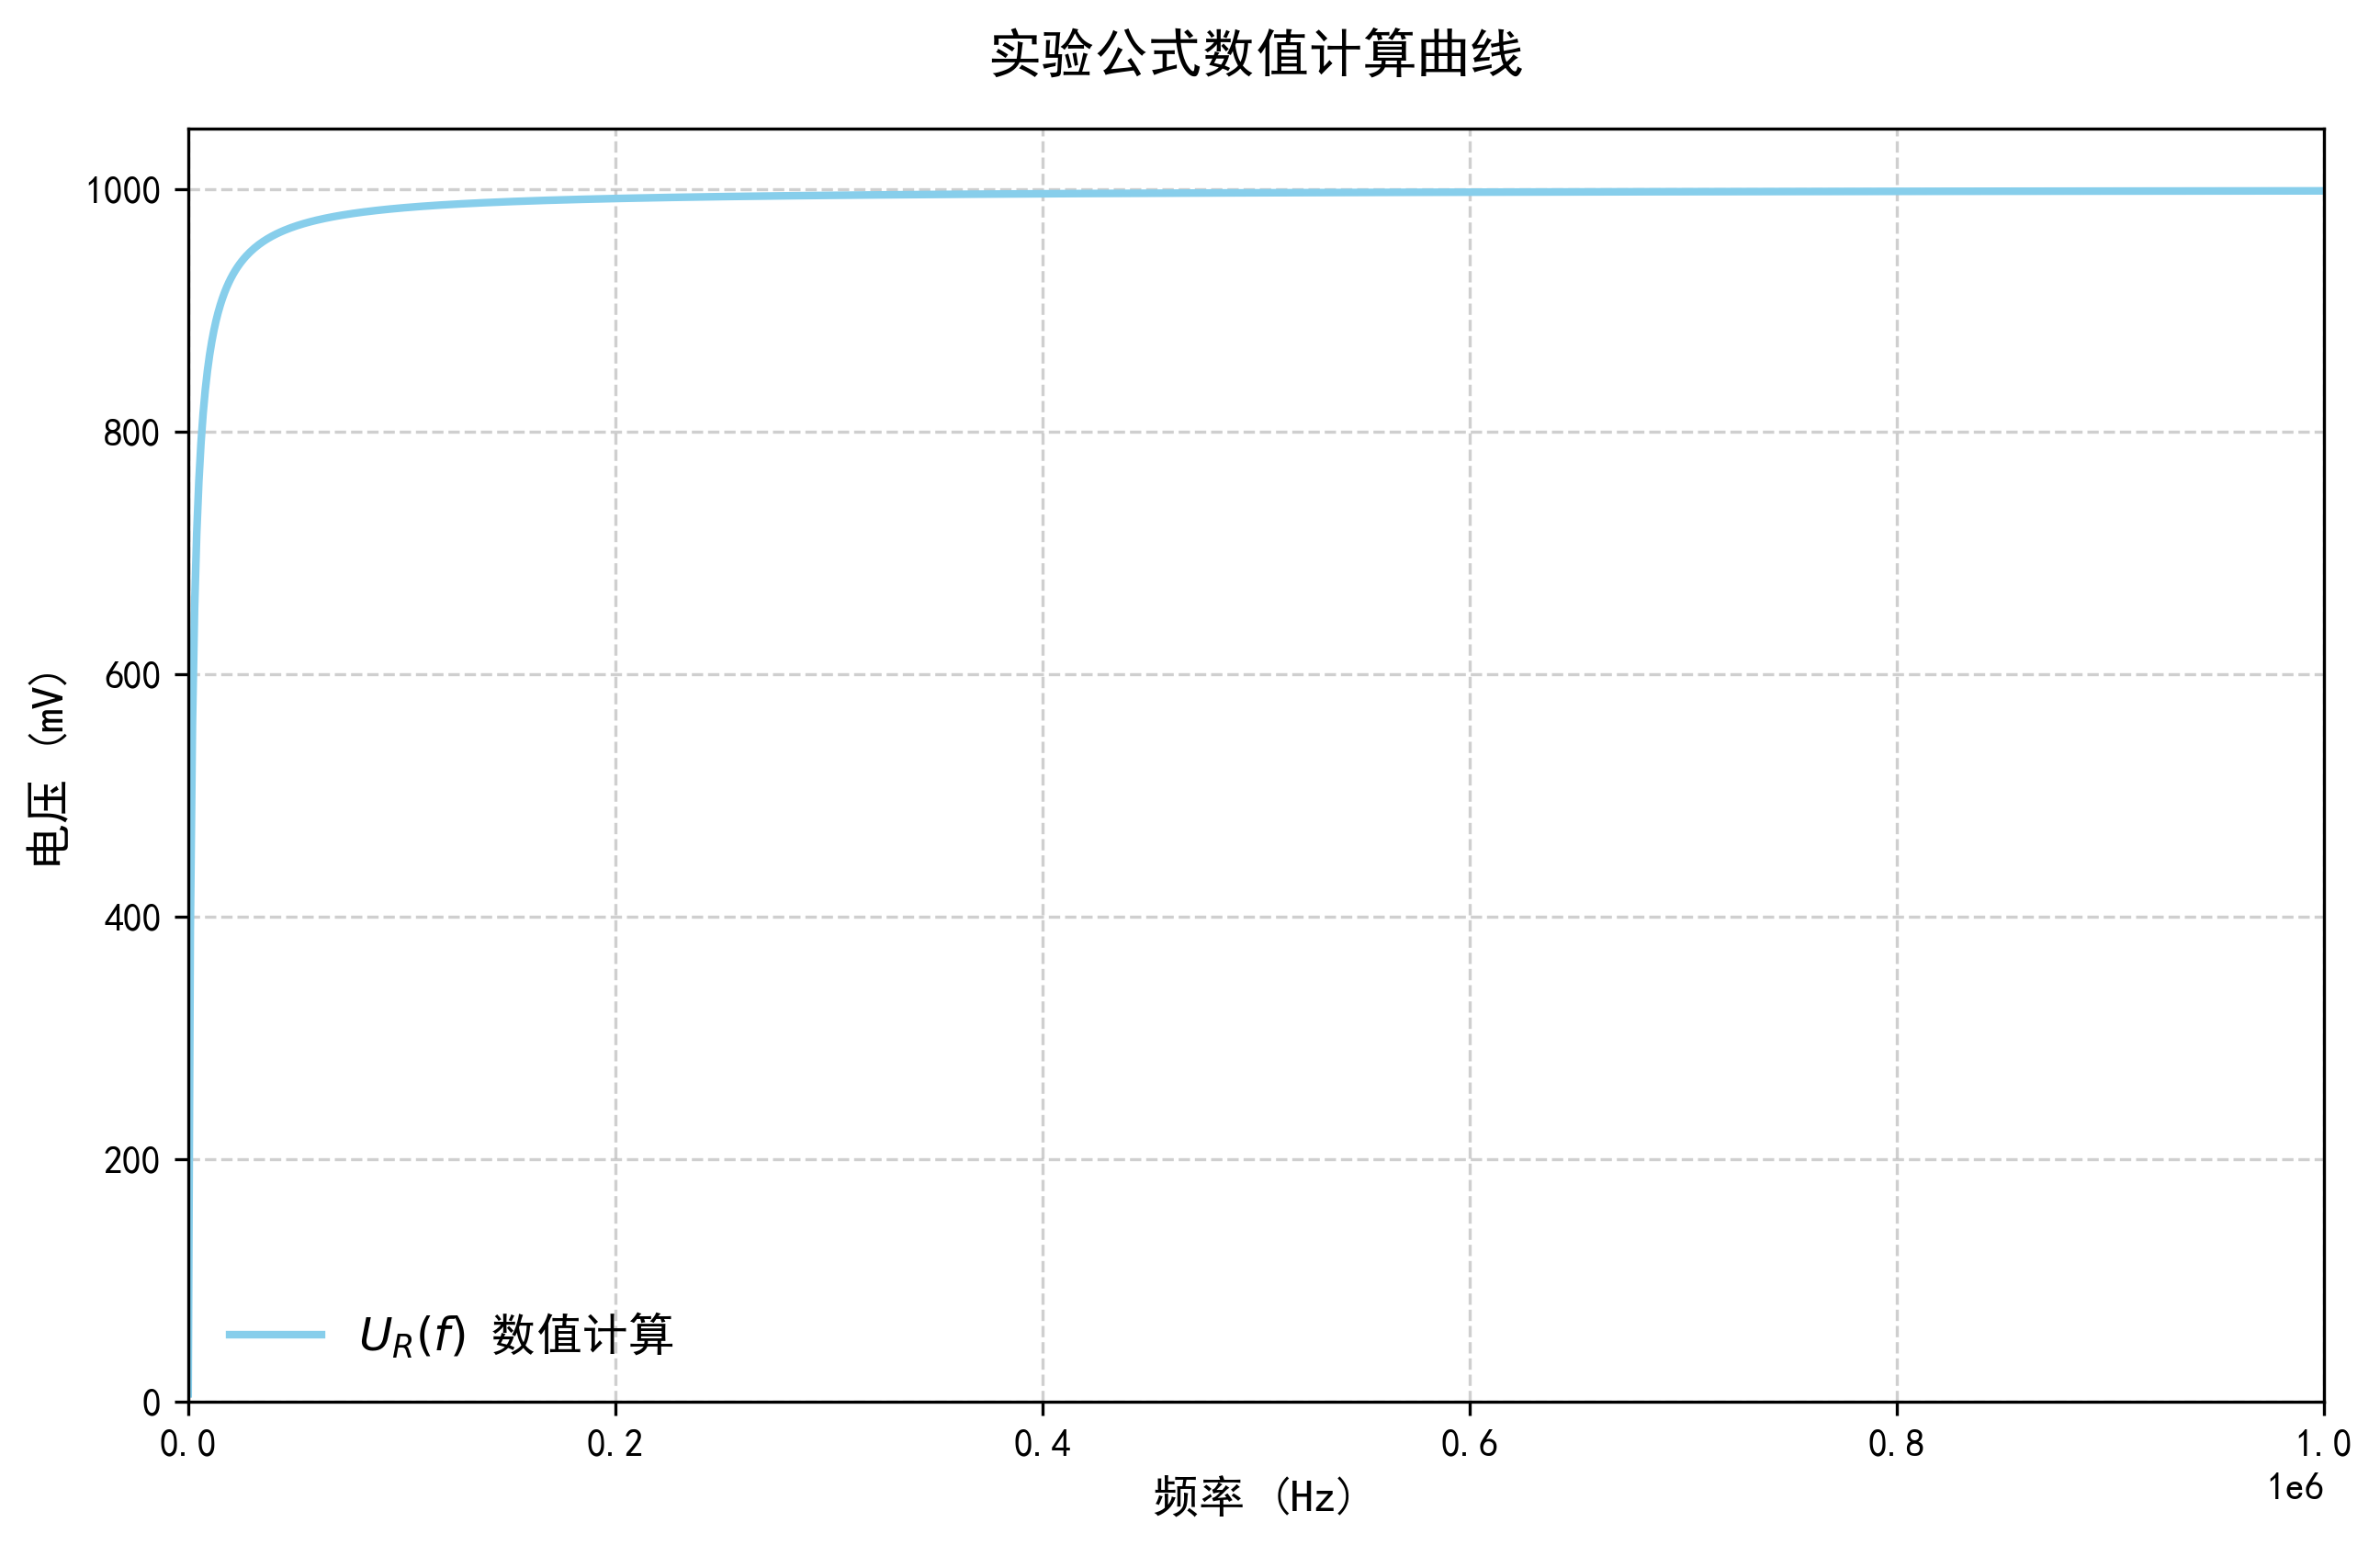
\includegraphics[width=0.65\textwidth]{python/UR_vs_f.png}
%   \caption{数据处理曲线（写明图名）}
%   \label{fig:result-curve}
% \end{figure}

% ====================== 六、实验结果与分析 ======================
\section{实验结果与分析（必填）}
（1. 给出完整的实验结果表达式 $X = \bar{x} \pm u$（注明单位）：
不确定度有效位一般取一位并采用进位法，测量值末位与不确定度末位对齐；
2. 有理论值或约定真值时，计算绝对误差与相对误差，判断结果是否在误差范围内；
3. 结合曲线与数据分析实验现象、规律及误差来源（系统误差、随机误差、方法误差等）。）

\subsection{实验结果}
（示例格式：$I = (1.6 \pm 0.4)\,\mathrm{A}$。）

\subsection{结果分析与误差分析}
\begin{itemize}
  \item 
  \item 
\end{itemize}

% ====================== 七、讨论、心得 ======================
\section{讨论、心得}
（对实验内容、现象和过程作小结；解答老师布置的思考题、探究题——请先写题干再作答；
记录实验中的收获、遇到的问题、原因分析及改进建议。）

\subsection{思考题}
% \subsubsection{（抄写思考题题干）}
% （在此作答。）

\subsection{实验心得}
\begin{itemize}[label=\textbullet]
  \item 
  \item 
\end{itemize}

\end{document}

% =====================================================
% 以下为常用插图模板，需要时复制到正文并取消注释
% =====================================================

%单图模板
%\begin{figure}[H]
%  \centering
%  \includegraphics[width=0.6\textwidth]{resource/data1.png}
%  \caption{图名}
%  \label{fig:single}
%\end{figure}

%双图并排模板
%\begin{figure}[H]
%  \centering
%  % 左图
%  \begin{subfigure}{0.48\textwidth}
%    \centering
%    \includegraphics[width=\textwidth]{resource/实验电压频率图1.png}
%    \caption{子图名（一）}
%    \label{fig:sub-1}
%  \end{subfigure}
%   \hspace{0.025\textwidth}
%  % 右图
%  \begin{subfigure}{0.48\textwidth}
%    \centering
%    \includegraphics[width=\textwidth]{resource/实验电压频率图2.png}
%    \caption{子图名（二）}
%    \label{fig:sub-2}
%  \end{subfigure}
%  \caption{总图名}
%  \label{fig:double}
%\end{figure}
